\section{Cluster-based Modal Analysis and Optimal Clustering}
\label{sec:problem}
In this section, we will describe the cluster-based modal analysis approach with focus on the optimization of clustering. Before we formulate this clustering problem, the basic concept of modal parameters, the techniques adopted for modal analysis and assembling method are described. Table \ref{tab:Table1} summarizes the notations used in this paper.

\begin{table}
	\centering
\begin{tabular}{|c|l|}
\hline
\(\mathbf{\Psi_k}\)& The \(k^{th}\) mode shape vector of the structure\\
\hline
\(p\) &	The number of mode shape vectors to be identified\\
\hline
\(G_{xy}(\omega)\)& The cross spectral density (\(x\neq y\))\\
\ & and power spectral density (\(x=y\))\\
\hline
\(N\) & the total data amount\\
\hline
\(M,c,n_i\) & the total number of sensor nodes,\\ 
\ & the number of generated clusters, \\
\ & and the number of sensor nodes in cluster \(S_i\)\\
\hline
\(n_t\)	& Length of each section to calculate CSD\\
\hline
\(n_d\)	& Number of averages\\
\hline
\(e_S, e_R, e_T \)& Energy consumed for sampling/rece./trans. one data\\
\hline
\(e_{NExT}, e_{ERA}\)	& Energy consumed for NExT and ERA\\
\hline
\end{tabular}
	\caption{Summary of Notations}
	\label{tab:Table1}
\end{table}

\subsection{Structural Mode Shapes}
In this section, we will give a brief introduction of one important type of modal parameters: mode shapes. 

Each mechanical structure has a number of specific vibration patterns at specific frequencies. These vibration patterns are called mode shapes. For example, we deploy a total of \(m\) sensor nodes on a structure and extract a total of \(p\) mode shapes from the measurement of these sensors:

\begin{equation}
[\mathbf{\Psi_1}, \mathbf{\Psi_2}, \cdots, \mathbf{\Psi_p}]=
\begin{bmatrix}
\phi_{11} & \phi_{12} & \cdots & \phi_{1p}\\
\phi_{21} & \phi_{22} & \cdots & \phi_{2p}\\
\vdots  & \vdots  & \ddots & \vdots  \\
\phi_{m1} & \phi_{m2} & \cdots & \phi_{mp}
\end{bmatrix} 
\end{equation}
where mode shape \(\mathbf{\Psi_k}=[\phi_{1k}, \phi_{2k}, \cdots, \phi_{mk}]'\) is the \(k^{th}\) vibration pattern of the structure.  \(\phi_{ik}(i=1,2,\cdots ,m)\) is the \(k^{th}\) mode shape value defined at the \(i^{th}\) sensor.

As an example, Fig. \ref{fig:modes} illustrates the first three mode shapes of a typical cantilevered beam, extracted from the measurements of the deployed 12 sensor nodes. 

\begin{figure}
\centering
\subfloat[]{\label{fig:originalbeam}
%\figurecurrentwidth{originalbeam}}
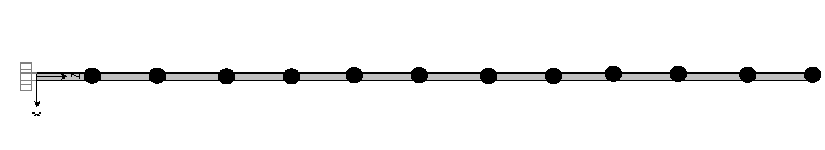
\includegraphics[width=.23\textwidth, height=0.05\textwidth]{originalbeam}}
%\qquad
\subfloat[]{\label{fig:mode1}
%\figurecurrentwidth{mode1}}
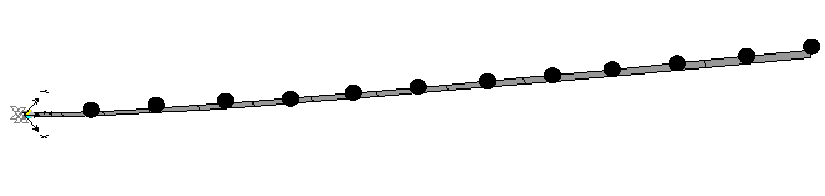
\includegraphics[width=.23\textwidth, height=0.05\textwidth]{mode1}}
\qquad
\subfloat[]{\label{fig:mode2}
%\figurecurrentwidth{mode2}}
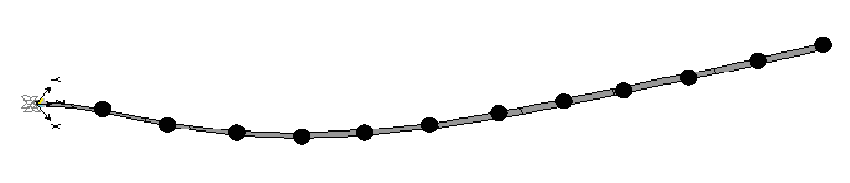
\includegraphics[width=.23\textwidth, height=0.05\textwidth]{mode2}}
%\qquad
\subfloat[]{\label{fig:mode3}
%\figurecurrentwidth{mode3}}
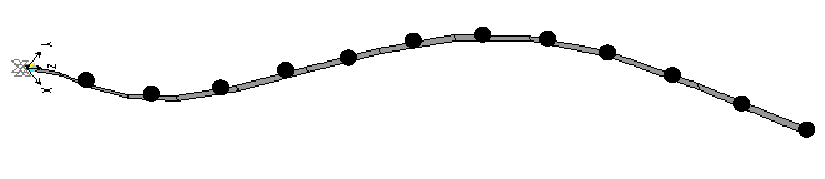
\includegraphics[width=.24\textwidth, height=0.05\textwidth]{mode3}}
%\qquad
%\subfloat[Mode 4 (Freq.=30.8Hz)]{\label{fig:mode4}
%\figurecurrentwidth{mode4}}
%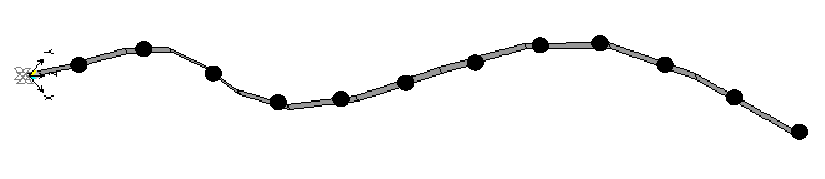
\includegraphics[width=.49\textwidth, height=0.05\textwidth]{mode4}}
\caption{Mode shapes of a typical cantilevered beam (a) Original beam (b)Mode Shape 1 (c) Mode Shape 2(d) Mode Shape 3}
\label{fig:modes}
\end{figure}

It can be seen that mode shape vector \(\mathbf{\Psi_k}\) has an element corresponding to each sensor node. The more number of sensor nodes used, the more elements are contained in \(\mathbf{\Psi_k}\), and more accurately this vibration pattern of the structure is described. Considering example in Fig. \ref{fig:modes}, if we double the number of nodes deployed on the beam, the vibration patterns will be represented with higher granularity. Another important characteristic of mode shape is that elements in \(\mathbf{\Psi_k}\) only represent the relative vibration amplitudes of structure at corresponding sensor nodes. That is, \(\mathbf{\Psi_k}=\zeta \mathbf{\Psi_k}\), where \(\zeta\) is any non-zero real number. This property will be re-visited when we formulate the clustering problem in section \ref{sec:OptimalClustering}.

\subsection{Cluster-based Modal Analysis and Its Energy Consumption}
In this section, we first give an overview of this cluster-based approach and then formulate the energy consumption of cluster-based modal analysis.

In the cluster-based modal analysis, deployed sensor nodes are partitioned into a number of single-hop clusters and each CH performs intra-cluster modal analysis to extract local mode shapes. Since mode shapes of a cluster only contain elements corresponding to the sensor nodes in that cluster, the mode shapes in all the clusters need to be assembled to obtain the mode shapes defined on all the deployed sensor nodes. The whole process is illustrated in Fig. \ref{fig:clusterflow}.

\begin{figure}
	\centering
		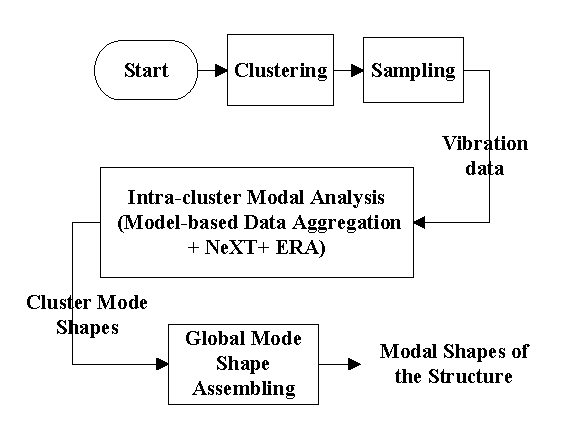
\includegraphics[width=.3\textwidth,height=.2\textwidth]{clusterflow.eps}
	\caption{Overview of cluster-based modal analysis process}
	\label{fig:clusterflow}
\end{figure}

In this paper, the modal parameters are identified using the natural excitation technique (NExT)\cite{james1993natural} in conjunction with the ERA. NexT+ERA is a widely accepted modal analysis approach and can give accurate mode shape estimate using output data-only. 

In each cluster, the NExT is used first to calculate power spectral density (PSD) of the CH and cross spectral density (CSD) between the CH and each of the cluster member. PSD and CSD functions are estimated using:
\begin{equation}
G_{xy}(\omega)=\frac{1}{n_d\cdot n_t}\sum\limits_{i=1}^{n_d}X_i^*(\omega)\cdot Y_i(\omega) \label{eq:next}
\end{equation}
where \(G_{xy}(\omega)\) is the CSD between two vibration signals, \(x(t)\) and \(y(t)\), measured from CH and a cluster member, respectively. \(X(\omega)\) and \(Y(\omega)\) are the Fourier transforms of \(x(t)\) and \(y(t)\), and '*' denotes the complex conjugate. \(n_t\) is time length of each record \(x_i(t)\) or \(y_i(t)\). \(n_d\) is the number of averages mainly for denoising purpose and \(n_d\) practically ranges from 10 to 20. When calculating \(G_{xy}\), consecutive records of \(x_i(t)\)(also \(y_i(t)\)) generally overlap. When \(y(t)\) in Eq. \ref{eq:next} is replace by \(x(t)\), the power spectral density (PSD) of CH is obtained. 

After obtaining CSD and PSD functions, the inverse Fourier transform is implemented and the cross-correlation functions (CCFs) and auto-correlation function (ACF) are obtained.  The ERA uses these functions to build a state space system whereby mode shapes of the structure are identified.

Traditionally, CH collects the raw data from all its cluster members, calculates CSDs and its PSD, and then uses the ERA to identify mode shapes.  However, the model-based data aggregation method proposed by \cite{nagayama2008structural} can be used here to decrease the energy consumption. In this approach, instead of collecting measurements data from cluster members, CH broadcasts its time record of length \(n_t\). On receiving the record, each cluster member calculates its CSD and stores it locally.  This procedure will be repeated \(n_d\) times, until the CSD is according to Eq. \ref{eq:next}. Each cluster member then transmits the first half of the corresponding CCF to the CH.
\begin{comment}
\begin{figure}
	\centering
		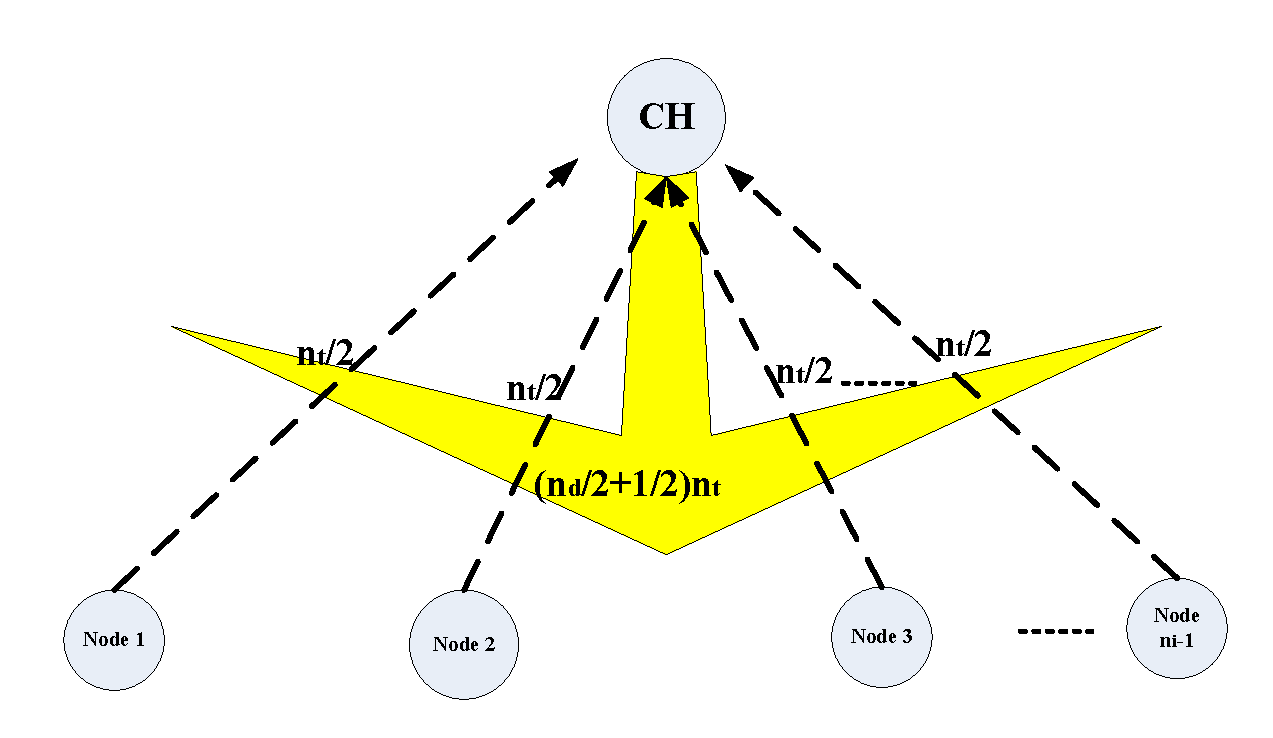
\includegraphics[width=.3\textwidth,height=.18\textwidth]{clusteraggregation.eps}
	\caption{Model-based data aggregation (Assume 50 \% Overlap)}
	\label{fig:clusteraggregation}
\end{figure}
\end{comment}

Based on the discussion above, we can estimate the energy consumption of intra-cluster modal analysis. To obtain the mode shapes of a cluster \(S_i\), the total energy consumption in \(S_i\), denoted as \(cost(S_i)\), can be mainly decomposed into the following three parts: 
\begin{subequations}
\begin{equation}
cost(S_i)=Er_s(S_i)+Er_c(S_i)+Er_a(S_i)
\end{equation}

where \(Er_s(S_i)\), \(Er_c(S_i)\)  and \(Er_a(S_i)\) are the energy consumed in data sampling, intra-cluster wireless communication and computation associated with modal analysis, respectively. 

Assume a cluster \(S_i\) contains a total of \(n_i\) sensor nodes, then sampling cost \(Er_s(S_i)\) is:
\begin{equation}
Er_s(S_i)=n_i\cdot N\cdot e_S
\end{equation}

where \(N\) is the total amount of time history record sampled in each sensor. Assuming 50 \% overlapping,  \(N=(n_d/2+1/2)n_t\). \(e_S\) is the energy for sampling one data. We assume that \(n_d\) , \(n_t\), \(N\) and \(e_S\) are fixed in this paper.  

The intra-cluster wireless communication cost \(Er_c(S_i)\) is:
\begin{align}
Er_c(S_i)=&N\cdot e_T+(n_i-1)N\cdot e_R\nonumber \\
+&(n_i-1)\frac{n_t}{2}(e_T+e_R) \label{eq:energytotal}
\end{align}
where \(e_T\) and \(e_R\) are the energy cost for transmitting and receiving one data, respectively. The first two terms at the right side of Eq. \ref{eq:energytotal} are the energy consumed when CH broadcasts its time history data and when all the cluster members receive the broadcasts, respectively. The last term is the energy consumption when the \((n_i-1)\) cluster members transmit back their correlation functions to the CH.

The computation cost \(Er_a(S_i)\) can be formulated as:
\begin{equation}
Er_a(S_i)=n_i\cdot e_{NExT}+e_{ERA}(n_i)
\end{equation}
\end{subequations}

where \(e_{NExT}\) is the energy consumed when each node implements the NExT (including calculating the CSD/PSD and CCF/ACF) and \(e_{ERA}\) is the energy used in CH when it carries out the ERA for mode shape identification. \(e_{NExT}\) is fixed given  \(n_t\) and \(n_d\). \(e_{ERA}\) is dependent on \(n_i\) and number of mode shape vectors \(p\) to be identified.  Given \(p\), \(e_{ERA}(n_i)\) is not a linear function of \(n_i\) since the ERA involves complex matrix computations including SVD and matrix inversion. This point is demonstrated in Fig. \ref{fig:ERAcomplexity}, where the computation time of our SHM mote to implement the ERA for different cluster sizes is illustrated. The fitting function is also illustrated in the figure. It can be seen that with the increase of \(n_i\), the time consumed, which is the indicator of energy consumption, is quadratically increased.
\begin{figure}
	\centering
		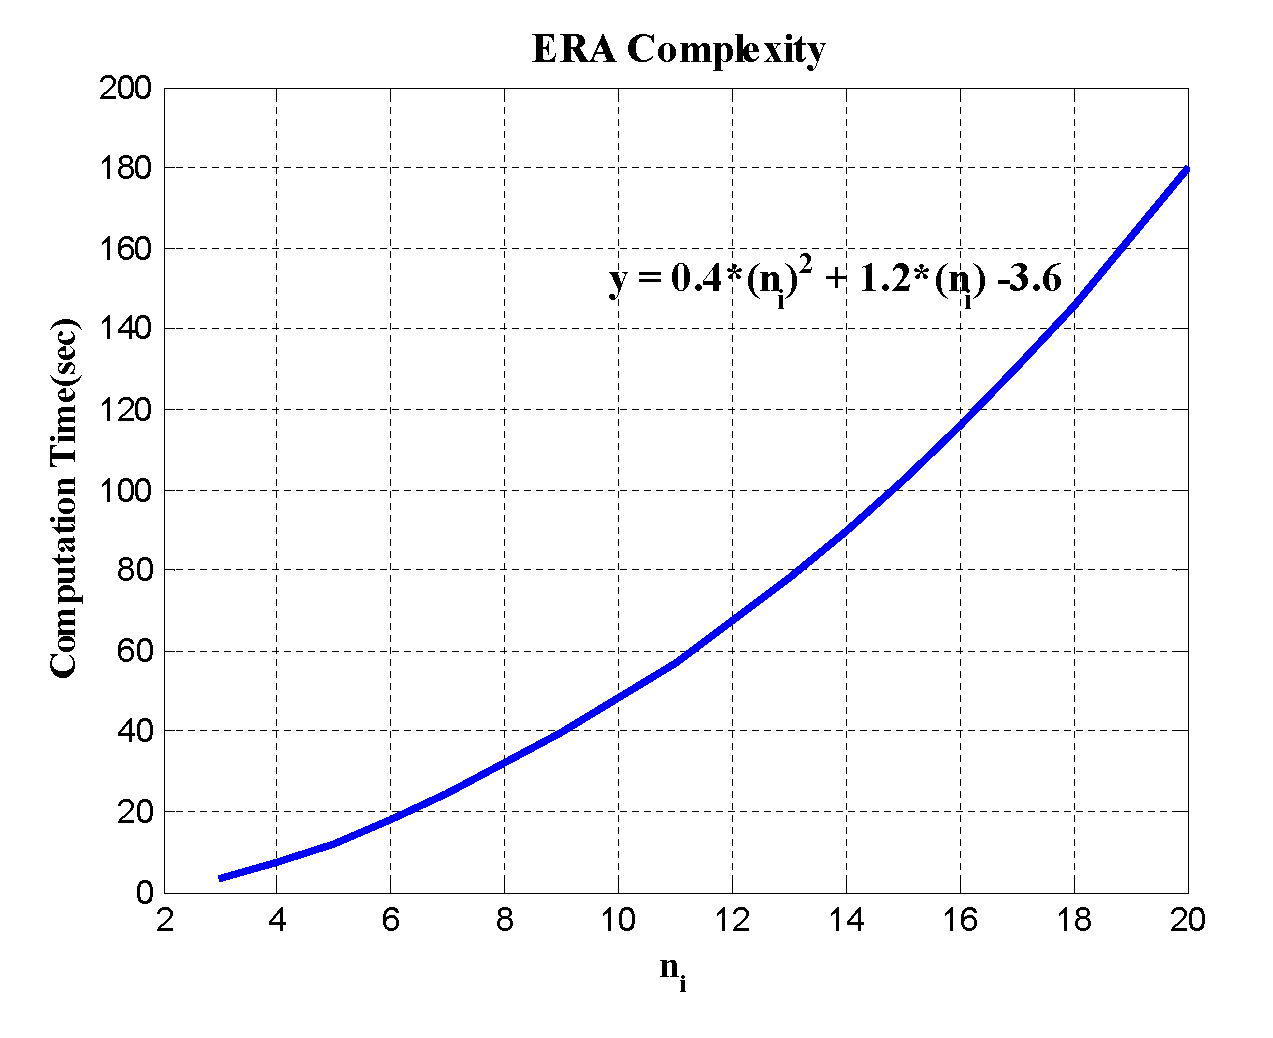
\includegraphics[width=.28\textwidth,height=.20\textwidth]{ERAcomplexity.eps}
	\caption{The complexity of the ERA}
	\label{fig:ERAcomplexity}
\end{figure}

From the equations above, we have \(cost(S_i)=cost(n_i)\), indicating that the energy consumption of a cluster is only associated with the number of sensor nodes in this cluster. It is of interest to see that if possible, whether to generate small-sized clusters or large-sized clusters is more energy efficient.  To find the answer, we assume \(M\) sensor nodes can be partitioned into equal-sized clusters of size \(n\), then the number of clusters \(c = M/n\). The optimal cluster size, denoted as \(n_{opt}\), can be obtained by looking for the \(n\) that minimizes the average energy consumption per node defined as: 

\begin{align}
\label{eq:nooverlap}
Epn(n) = \frac{c\cdot cost(n)}{M} = N(e_S+\beta) + e_{NExT}\\ \nonumber 
+ \frac{N(e_T-\beta)}{n} + \frac{e_{ERA}(n)}{n} 
\end{align}
where \(\beta =e_R+\frac{n_t}{2N}(e_T+e_R)\).

The \(3^{rd}\) term in the right side of the Eq. \ref{eq:nooverlap} indicates that in terms of wireless communication, partitioning sensor network into large-sized clusters is preferred when \(e_T \geq \beta\) while generating small-sized clusters is better if otherwise. The \(4^{th}\) term tells us that small cluster size \(n\) is more energy efficient in terms of computation considering that \(e_{ERA}(n)\) is a quadratic function of \(n\). As a result, there does not exist a rule of thumb for clustering and we have different optimal cluster sizes for different conditions. As an example, some parameters obtained by some real tests of our SHM Mote are listed in Table \ref{tab:Table2}. Based on Table \ref{tab:Table2}, Fig. \ref{fig:MagicNumber2}a shows various optimal cluster sizes, illustrated as red dots in the figure, when the transmission power \(e_T\) is set to be from \(e_T = e_R\) to \(e_T = 5 e_R\). It can be seen that when \(e_T=e_R\), the smaller the cluster size, the better. (Note that the ERA requires that the number of sensor nodes in each cluster should be at least larger than \(p\)). With the increase of \(e_T\), the optimal cluster size is increased but does not go unbounded considering the energy consumption of the ERA for large-sized clusters.

\begin{figure}
	\centering
		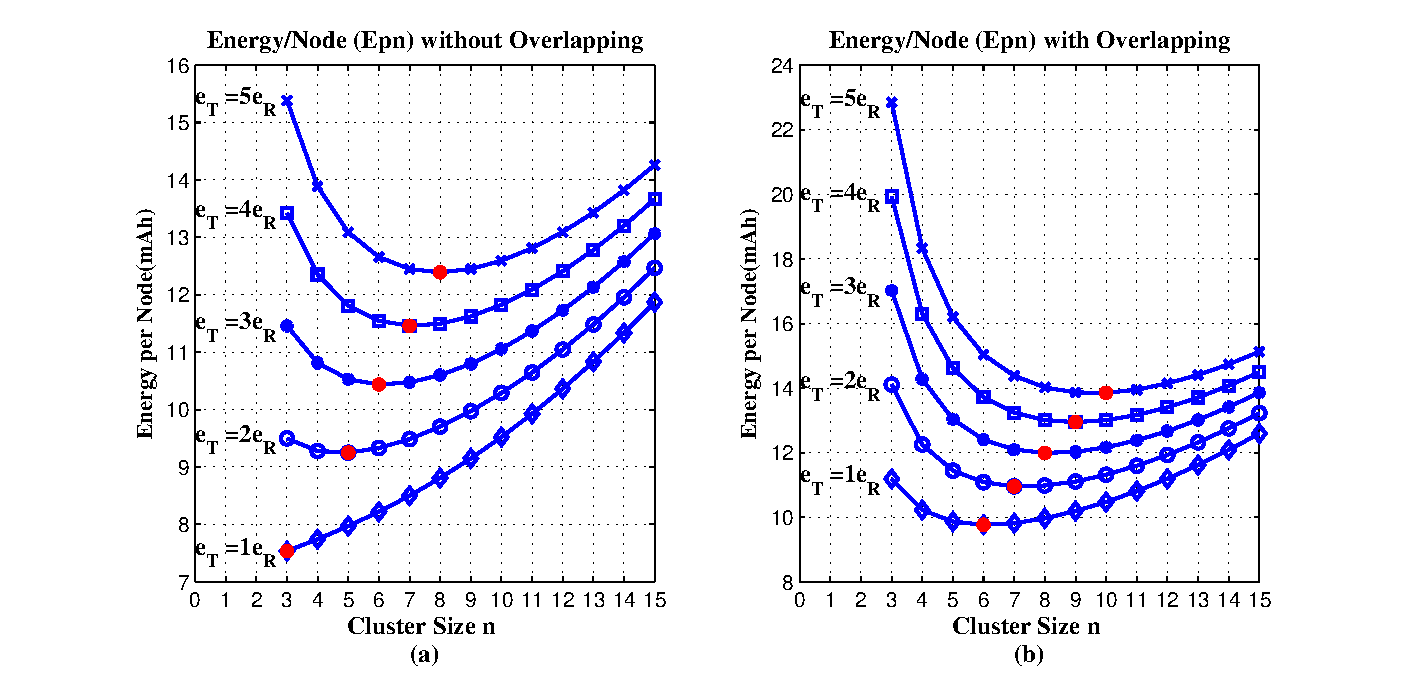
\includegraphics[width=.5\textwidth,height=.25\textwidth]{EnergyPerNode.eps}
	\caption{The optimal cluster sizes in different conditions. (a)No overlapping (b)with overlapping}
	\label{fig:MagicNumber2}
\end{figure}


\begin{table}
	\centering
\begin{tabular}{|c|c|c|c|c|c|c|c|}
\hline
\(N\)&\(p\)&\(n_t\)&\(n_d\)&\(e_S\)&\(e_R\)&\(e_{NExT}\)&\(e_{ERA}\)\\
& & & &(mAh)&(mAh)&(mAh)&(mAh)\\
\hline
     &     &       &       &       &   & &\(0.0417(0.4n_i^3\)\\
10752&3&1024&20&1.1e-4&5e-4&0.5&\(+1.2n_i\)\\
&&&&&&&-3.6)\\
\hline
\end{tabular}
	\caption{Parameters used in Fig. \ref{fig:MagicNumber2}}
	\label{tab:Table2}
\end{table}

Clustering using minimum dominating set \cite{wan2004distributed} or maximum independent set 
\cite{banerjee2001clustering} cannot be directly applied to solve our clustering problem since they mainly aim to find as small number of clusters as possible. Also, in the discussion so far, we assume that no overlapping nodes exist in the clusters. However, we will show in the following section that a necessary condition for cluster-based modal analysis is that all the generated clusters must be connected through the overlapping nodes. This requirement further increases the difficulty of the clustering problem.

\subsection{Determination of Global Mode Shapes through Mode Shape Assembling}
After the mode shapes in all clusters have been identified, they need to be stitched together to obtain mode shapes defined on all of deployed sensor nodes. 

However, since mode shape vectors identified in a cluster only represent the relative vibration amplitudes at cluster sensor nodes, mode shapes of different clusters may not be able to be assembled together. This can be demonstrated in Fig. \ref{fig:TwoTypesClustering}a, where the deployed 12 sensor nodes in Fig. \ref{fig:modes} are partitioned into three clusters to identify the \(3^{rd}\) mode shape.  Although the mode shape of each cluster is correctly identified, we still cannot obtain the mode shapes for the whole structure. The key to solve this problem is overlapping.  We must ensure that each cluster has at least one node which also belongs to another cluster and all the clusters are connected through the overlapping nodes (a more formal definition will be given in the next section).  For example, in Fig. \ref{fig:TwoTypesClustering}\((b)\), mode shapes identified in each of the three clusters can be assembled together with the help of the overlapping nodes \(5\) and \(9\). This requirement of overlapping must be satisfied when formulating the problem of optimal clustering.

\begin{figure}
\centering
\subfloat[]{\label{fig:NonOverlapClusterBeam}
%\figurecurrentwidth{originalbeam}}
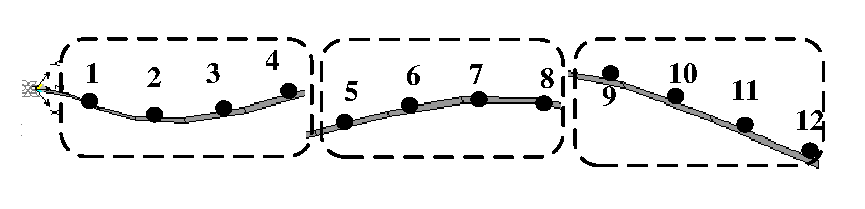
\includegraphics[width=.25\textwidth, height=0.08\textwidth]{NonOverlapClusterBeam}}
%\qquad
\subfloat[]{\label{fig:OverlapClusterBeam}
%\figurecurrentwidth{mode1}}
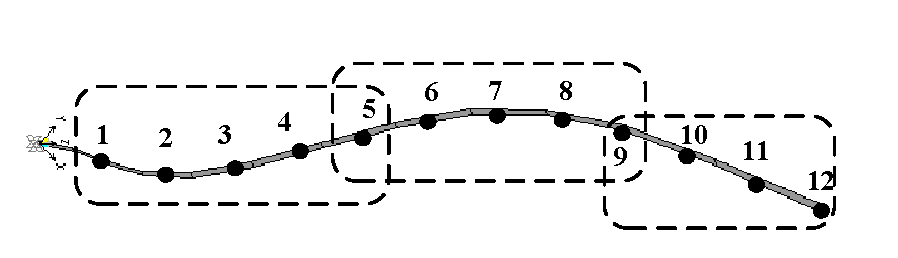
\includegraphics[width=.25\textwidth, height=0.08\textwidth]{OverlapClusterBeam}}
\caption{Mode shape assembling when (a) clusters do not overlap (b) clusters overlap}
\label{fig:TwoTypesClustering}
\end{figure}

It is obvious that overlapping will affect the overall energy consumption and consequently, the optimal cluster size \(n_{opt}\) will be different from that when no overlapping is considered.  By defining the number of overlapping nodes as \(n_o = \sum\limits_{i=1}^c\left|S_i\right| - M\), and still assume these \(M\) sensor nodes are partitioned into equal-sized clusters of size \(n\), then the energy consumption per node becomes

\begin{align}
\label{eq:MagicNumberOverlapping}
Epn'(n) = \frac{(M+n_o)/n \cdot cost(n)- n_o \cdot N \cdot e_S}{M}\\ \nonumber
=\frac{cost(n)}{n}  + \frac{n_o}{M} \cdot \kappa
\end{align}

where \(\kappa = N \cdot \beta + e_{NExT}+ \frac{N(e_T-\beta)}{n} + \frac{e_{ERA}(n)}{n}\).  Considering the fact that unnecessary overlapping will cause extra energy consumption and the number of overlapping nodes should be kept as small as possible, we require that \(n_o \geq \frac{M+n_o}{n} -1\). Therefore,

\begin{equation}
\label{eq:MagicNumberOverlapping2}
Epn'(n) \geq \frac{cost(n)}{n}+ \frac{1-n/M}{n-1}\kappa
\end{equation}

The right side of Eq. \ref{eq:MagicNumberOverlapping2} essentially provides a lower bound of energy consumption that clustering can achieve when the overlapping constraint is considered. The optimal cluster size \(n_{opt}\) can be calculated by minimizing \(n\) in Eq. \ref{eq:MagicNumberOverlapping2}.  For example, the \(n_{opt}\) for the parameters listed in Table \ref{tab:Table2} are illustrated in Fig. \ref{fig:MagicNumber2}b. 

By comparing Fig.\ref{fig:MagicNumber2}a with Fig.\ref{fig:MagicNumber2}b, it also can be easily seen that optimal cluster size is larger when overlapping constraint is considered. Clustering which generates small-sized clusters may not be energy efficient since a large number of overlapping nodes can cause extra energy consumption in terms of communication and computation. 

Also should be noted is that the optimal cluster size \(n_{opt}\), either obtained by Eq. \ref{eq:nooverlap} or by Eq. \ref{eq:MagicNumberOverlapping2}, is not affected by actual network topology. In a dense network, it is more possible to achieve the obtained optimal cluster size and therefore, the total energy will be lower than a sparse network.

We do not consider the inter-cluster communication in this paper simply because delivering obtained mode shapes requires significantly less energy than other processes.

\subsection{Optimal Clustering}
\label{sec:OptimalClustering}
In this section, we will formulate the optimal clustering problem.  The objective of clustering is that the generated clusters can minimize the energy consumption of overall modal analysis. Clustering also has to satisfy the following constraints (1) each sensor node belongs to at least one of the generated clusters, (2) sensor nodes in each cluster is within a single communication range to its CH, (3) number of sensor nodes in each cluster is larger than \(p\) (\(p\):the number of mode shape vectors to be identified) (4) all the clusters are connected together through the overlapping nodes. More formally, problem is formulated as follows:
Given a sensor network \(G=(V,E)\), find a clustering scheme that can cluster these \(V\) sensor nodes into a set of clusters, denoted as \(C=\{S_1, S_2, S_3, \cdots\}\), subject to the following constraints:
\begin{enumerate}
	\item \( \bigcup\limits_{S_i \in C} = V\)
	\item Let the sub-graph for \(S_i\) is \(G(S_i,E_i)\), where \(E_i \subseteq E\). Then \(\forall S_i \in C, \exists s_i \in S_i\), such that there is an edge \(a_{ij} \in E_i\) between \(s_i\) and any other \(s_j \in S_i (s_i \neq s_j)\) 
	\item \(\forall S_i \in C, \left|S_i\right|\geq p\)
	\item \( \forall S_i, \exists S_j \in C, (i \neq j), S_i \bigcap S_j \neq \emptyset\)
	\item \(\forall C' \subseteq C, (\bigcup\limits_{S_i \in C'} S_i)\bigcap (\bigcup\limits_{S_j \in C-C'} S_j) \neq \emptyset \)
\end{enumerate}
Objective:
\begin{itemize}
\item Minimize \(\sum\limits_{S_i \in C} cost(S_i)\)
\end{itemize}

The first constraint is set because we wish to find the mode shapes defined on all the deployed sensor nodes. The second constraint is to ensure only single-hop clusters are generated. Constraint 3 is required by the ERA algorithm. Constraints 4 and 5 are used to describe that generated clusters are overlapping and connected. 

The above clustering problem is an optimization problem. We will prove that the decision version of the problem is NP complete which is defined as: \emph{given a threshold \(k\) , does there exist a cluster set \(C=\{S_1, S_2, S_3, \cdots\}\), which satisfy all the constraints above and whose total energy cost \(\sum\limits_{S_i \in C} cost(S_i)\) is equal of smaller than \(k\)?}.

\begin{theorem}
The decision version of our clustering problem is NP-complete.
\end{theorem}

\begin{proof}
It is easy to find out this clustering problem is NP.  Given a cluster set \(C\), all the constraints above, include constraints 4 and 5 can be checked in a polynomial time. The detailed proof of this part is omitted for brevity.

We show this decision version of the clustering problem is NP-hard by reducing the set cover problem to it. The set cover problem is defined as follows.

\begin{flushleft}
\textbf{Given:}
\end{flushleft}
\begin{enumerate}
\item A universe \(V'\)
\item A set of \(S'=\{S'_1, S'_2, ...\}\subseteq V'\)
\item The cost function for each subset \(S'_i\in S'\): \(cost'(S'_i)\) 
\item A number \(k'\)
\end{enumerate}
\textbf{Find: }
If there is a subset \(C'\subseteq S'\) which satisfies
\begin{enumerate}
\item \( \bigcup\limits_{S'_i \in C'} S'_i =V'\)
\item \( \sum\limits_{S'_i \in C'} cost'(S'_i) \leq k'\)
\end{enumerate}

To reduce the set cover problem to the clustering problem, we construct a sensor network \(G=(V, E)\) from the inputs of set cover problem in the following way:
The vertices \(V =V'\bigcup X\) , where \(X = \{x_1,x_2,...x_p\}\)  is a set of \(p\) virtual nodes. 
To construct the edges \(E\), for each \(S'_i\in S'\) , we first choose an arbitrary  node \(s'_i\in S'_i\), then we add an edge between \(s'_i\) and any other node \(s'_j \in S'_i (s'_j\neq s'_i)\). We also add an edge between \(s'_i\) and any virtual node in \(X\). 
The cost function in the clustering problem \(cost(\cdot) = cost'(\cdot)\). We also define that by adding/deleting any virtual node \(x\) to/from any group will not affect the cost function. The energy threshold \(k=k'\). 

With this transformation, it can be easily proved that 1) Assume \(C'=\{S'_1, S'_2, ...\}\)is a solution to the set cover problem, then \(C=\{S_1, S_2, ...\}\)  is a solution to the clustering problem, where \(S_i = S'_i \bigcup X\). 2) Assume \(G =(V,E)\) is constructed from the set cover problem and we have a solution \(C=\{S_1, S_2, ...\}\) to the clustering problem, then \(C'=\{S'_1, S'_2, ...\}\) is a solution to the set cover problem, where \(S'_i=S_i - X\). The detailed proof is omitted for brevity. 
\end{proof}
By reducing the NP-complete set problem to our clustering problem, we have demonstrated that the decision version of our problem is NP-complete. Obviously, the original clustering problem is also NP-Complete.